
\documentclass[aspectratio=169,xcolor=dvipsnames]{beamer}

\usetheme{default}
\usefonttheme[onlymath]{serif}

\beamertemplatenavigationsymbolsempty

\usepackage{hyperref}
\usepackage{graphicx}
\usepackage[usexcolor=false]{svg}
\usepackage{booktabs} % Allows the use of \toprule, \midrule and \bottomrule in tables
% \usepackage{tikz}
% \usepackage{pgfplots}

\usepackage{slideshow}

%----------------------------------------------------------------------------------------
%	TITLE PAGE
%----------------------------------------------------------------------------------------

% The title
\title[short title]{Variables in System Dynamics}
\subtitle{an introduction}

\author[Rico A.R.\ Picone] {Rico A.R.\ Picone}
\institute[SMU] % Your institution may be shorthand to save space
{
    % Your institution for the title page
    Department of Mechanical Engineering \\
    Saint Martin's University
    \vskip 3pt
}
\date{\today} % Date, can be changed to a custom date


%----------------------------------------------------------------------------------------
%	PRESENTATION SLIDES
%----------------------------------------------------------------------------------------

\begin{document}

\begin{frame}
\maketitle
\end{frame}

%------------------------------------------------
%------------------------------------------------

\begin{frame}{Variables represent quantities}
    % This file was created by matlab2tikz.
%
\definecolor{mycolor1}{rgb}{0.00000,0.44700,0.74100}%
\definecolor{mycolor2}{rgb}{0.85000,0.32500,0.09800}%
%
\begin{tikzpicture}

\begin{axis}[%
width=0.856\linewidth,
height=0.33\linewidth,
at={(0\linewidth,0\linewidth)},
scale only axis,
xmin=0,
xmax=5,
xlabel style={font=\color{white!15!black}},
xlabel={time},
ymin=-3,
ymax=5,
ylabel style={font=\color{white!15!black}},
ylabel={variables through time},
axis background/.style={fill=white},
xmajorgrids,
ymajorgrids,
legend style={legend cell align=left, align=left, draw=white!15!black},
scaled ticks=false,tick label style={/pgf/number format/fixed}
]
\addplot [color=mycolor1, line width=1.5pt]
  table[row sep=crcr]{%
0	1\\
0.0499999999999998	2.05027061043666\\
0.0999999999999996	2.89857585853573\\
0.15	3.54453424996401\\
0.2	3.99248171253971\\
0.25	4.25151443792874\\
0.3	4.33528302296176\\
0.35	4.26156661151143\\
0.4	4.05166169988472\\
0.45	3.72962475821526\\
0.5	3.32141071146634\\
0.55	2.85395056197815\\
0.7	1.3604954750124\\
0.75	0.91271036578967\\
0.8	0.523621653476178\\
0.850000000000001	0.208283658910929\\
0.9	-0.0222395761430443\\
0.95	-0.161055856313822\\
1	-0.20546284707664\\
1.05	-0.156808763369605\\
1.1	-0.0202079196782599\\
1.15	0.195871495774502\\
1.2	0.48012582986515\\
1.25	0.819015794395222\\
1.3	1.19742091615006\\
1.45	2.40908406985178\\
1.5	2.78637842709068\\
1.55	3.12716622483295\\
1.6	3.42026954601979\\
1.65	3.65686900193463\\
1.7	3.83073735996894\\
1.75	3.93836018335446\\
1.8	3.97894441265274\\
1.85	3.95432011560782\\
1.9	3.86874451812499\\
1.95	3.72862077324758\\
2	3.54214662320285\\
2.05	3.3189100882333\\
2.1	3.069450532981\\
2.25	2.27388371208839\\
2.3	2.02821263535604\\
2.35	1.80781716708562\\
2.4	1.62006167305403\\
2.45	1.47067838616445\\
2.5	1.36362461651808\\
2.55	1.30101587410806\\
2.6	1.28313381249372\\
2.65	1.30850504412389\\
2.7	1.37404431342989\\
2.75	1.47525332780619\\
2.8	1.60646480565827\\
2.85	1.7611200507987\\
2.9	1.93206762824973\\
3.05	2.4686699594442\\
3.1	2.632005780029\\
3.15	2.7773641885324\\
3.2	2.89997187885537\\
3.25	2.9961727028116\\
3.3	3.06351540770588\\
3.35	3.10079023409791\\
3.4	3.10801544561732\\
3.45	3.08637675726542\\
3.5	3.03812431547209\\
3.55	2.96643330680699\\
3.6	2.87523539014714\\
3.65	2.76902893071459\\
3.7	2.65267644954931\\
3.8	2.4095672447599\\
3.85	2.29252236531809\\
3.9	2.18439127647949\\
3.95	2.08894435100673\\
4	2.00927479913895\\
4.05	1.94771141476031\\
4.1	1.90576530184057\\
4.15	1.88411099563293\\
4.2	1.8826010353917\\
4.25	1.90031179054767\\
4.3	1.93561723413\\
4.35	1.98628643168741\\
4.4	2.04959979812428\\
4.45	2.12247868633749\\
4.5	2.20162261822853\\
4.6	2.36522595851296\\
4.65	2.4432047722964\\
4.7	2.51472809790819\\
4.75	2.57732949850827\\
4.8	2.62900976676978\\
4.85	2.66829188061934\\
4.9	2.69425297269092\\
4.95	2.70653319137364\\
5	2.70532223589523\\
};
\addlegendentry{$v\ (V)$}

\addplot [color=mycolor2, line width=1.5pt]
  table[row sep=crcr]{%
0	-2\\
0.0499999999999998	-2.21404755936071\\
0.0999999999999996	-2.35343285280274\\
0.15	-2.41637698405024\\
0.2	-2.40416035031419\\
0.25	-2.32092364851451\\
0.3	-2.17336735925759\\
0.35	-1.97036634590932\\
0.4	-1.72251869557486\\
0.45	-1.44164955307829\\
0.5	-1.14029143716138\\
0.600000000000001	-0.526662390522305\\
0.65	-0.238406629097608\\
0.7	0.0231878487878943\\
0.75	0.249248813579539\\
0.8	0.432718516413652\\
0.850000000000001	0.568539647595617\\
0.9	0.653754435529738\\
0.95	0.687517268672128\\
1	0.671024567213964\\
1.05	0.607368667324046\\
1.1	0.501325105844604\\
1.15	0.359084825310144\\
1.2	0.187944399188991\\
1.25	-0.00403162919235545\\
1.4	-0.620160606942649\\
1.45	-0.811648340065915\\
1.5	-0.984108578333853\\
1.55	-1.13176291404044\\
1.6	-1.25007937256811\\
1.65	-1.33588785614137\\
1.7	-1.3874369985836\\
1.75	-1.4043930776088\\
1.8	-1.38778385283302\\
1.85	-1.33989219945754\\
1.9	-1.26410612234073\\
1.95	-1.16473311025236\\
2	-1.04678778858927\\
2.05	-0.915762430262269\\
2.2	-0.501343633316393\\
2.25	-0.37429156190422\\
2.3	-0.260754676412581\\
2.35	-0.164488895106172\\
2.4	-0.0883953437068818\\
2.45	-0.0344492292483096\\
2.5	-0.0036681886083878\\
2.55	0.00388058266520286\\
2.6	-0.0109634102102918\\
2.65	-0.0465308270611526\\
2.7	-0.100427879222839\\
2.75	-0.169664747574323\\
2.8	-0.25080091513953\\
2.85	-0.340100937834256\\
2.95	-0.527731466195752\\
3	-0.618534617910522\\
3.05	-0.702730252770265\\
3.1	-0.777366542528486\\
3.15	-0.840007351579451\\
3.2	-0.888801819323721\\
3.25	-0.922527789615857\\
3.3	-0.940608673964261\\
3.35	-0.943104388382112\\
3.4	-0.930677980767276\\
3.45	-0.904540432145252\\
3.5	-0.866376842739571\\
3.55	-0.818257781113885\\
3.6	-0.762539967320341\\
3.65	-0.701760672334015\\
3.75	-0.575427048681356\\
3.8	-0.514898741198585\\
3.85	-0.459173484465221\\
3.9	-0.410183995821342\\
3.95	-0.369506801856958\\
4	-0.33831830430586\\
4.05	-0.317368548120025\\
4.1	-0.30697284844904\\
4.15	-0.307020731133632\\
4.2	-0.317000994657997\\
4.25	-0.336041132734399\\
4.3	-0.362958884134071\\
4.35	-0.396323313714792\\
4.4	-0.434522584570689\\
4.5	-0.518503569786521\\
4.55	-0.56080160262322\\
4.6	-0.601102780928621\\
4.65	-0.637937317282968\\
4.7	-0.670041912509025\\
4.75	-0.696398810511512\\
4.8	-0.716263400057803\\
4.85	-0.729179848733188\\
4.9	-0.734984744797322\\
4.95	-0.73379919018405\\
5	-0.726010215365226\\
};
\addlegendentry{$i\ (A)$}

\end{axis}
\end{tikzpicture}%
    \note[itemize]{
        \item In dynamic systems and elsewhere, we use mathematical variables to represent physical quantities that change through time.
        \item Consider, for instance, an electronic system.
        \item This plot shows two traces through time, one for voltage and the other for current.
        \item The specific waveforms are determined by a number of things:
        \item the specific voltage and current being represented,
        \item the topology of the system,
        \item the system's initial conditions.
    }
\end{frame}

\begin{frame}{Power flow variables}
    For instance,
    \begin{equation}
        \underbrace{\mathcal{P}(t)}_{\text{power}} = \underbrace{i(t)}_{\text{current}} \underbrace{v(t)}_{\text{voltage}}.
    \end{equation}
    \note[itemize]{
        \item Here is the definition of power in an electronic system: the product of current and voltage.
        \item Power in all the domains we'll consider have the same form, the product of two variables.
        \item In each energy domain, a pair of variables will be called the power flow variables, and their product will be the power.
        \item The choice is not uniquely determined by their product being the power; however, there are common conventions we'll follow.
    }
\end{frame}

\begin{frame}{Through- and across-variables}
    \begin{center}
    \begin{tikzpicture}
        % \coordinate (g) at (-2.5,0);
        % \draw (g) pic {groundnode};
        % \node[above,font=\footnotesize] at (g) {ground};
        \node[graphnode] (n1) at (0,2) {};
        \node[graphnode] (n2) at (0,0) {};
        \draw[branch] (n1) to [bend left] (n2);
        \draw[->,>=stealth',thick,color=mygreen,line cap=round,bend angle=22] (0,1.5) to[bend left] (0,.5);
        \node[left=-3pt] at (0,1) {through-variable};
        \draw[thick,color=mygreen,line cap=round]
            ($(n1)+(.2,0)$) -- ++ (.6,0)
            coordinate (n12) -- ++(.15,0);
        \draw[thick,color=mygreen,line cap=round]
            ($(n2)+(.2,0)$) -- ++ (.6,0)
            coordinate (n22) -- ++(.15,0);
        \draw[->,thick,color=mygreen,line cap=round,>=stealth']
            (n12) -- node[midway,right,color=black] {across-variable} 
            node[midway,right,color=black,anchor=north west,font=\footnotesize] {drop} (n22);
        \node[graphnode] (n3) at (5,2) {};
        \node[graphnode] (n4) at (5,0) {};
        \draw[branch] (n3) to [bend left] (n4);
        \draw[->,>=stealth',thick,color=mygreen,line cap=round,bend angle=22] (0,1.5) to[bend left] (0,.5);
        \node[left=-3pt] at (5,1) {$i$};
        \draw[thick,color=mygreen,line cap=round]
            ($(n3)+(.2,0)$) -- ++ (.6,0)
            coordinate (n12) -- ++(.15,0);
        \draw[thick,color=mygreen,line cap=round]
            ($(n4)+(.2,0)$) -- ++ (.6,0)
            coordinate (n22) -- ++(.15,0);
        \draw[->,thick,color=mygreen,line cap=round,>=stealth']
            (n12) -- node[midway,right,color=black] {$v$} 
            node[midway,right,color=black,anchor=north west,font=\footnotesize] {drop} (n22);
    \end{tikzpicture}
    \end{center}
    \note[itemize]{
        \item In each energy domain, each of the pair of power flow variables has a unique type.
        \item One is called a through-variable. This variable passes through the element and is the same on both ends.
        \item We see this variable on the left of each diagram. In an electronic system, we see that this is the current $i$, which flows through the element and can be measured on either end.
        \item The other power flow variable is called an across-variable. This variable is defined as a relative quantity across the element and must be measured across the ends of the element. 
        \item The across-variable can be considered to ``drop'' across the element.
        \item We see this variable on the right of each diagram. In an electronic system, we see that this is the voltage $v$, which drops across the element and must be measured at both ends ends.
    }
\end{frame}

\begin{frame}{Electronic power flow variables}
    \begin{equation}
        \underbrace{\mathcal{P}(t)}_{\text{power}} = \underbrace{i(t)}_{\text{through}} \underbrace{v(t)}_{\text{across}}.
    \end{equation}
    \begin{center}
    \begin{circuitikz}[]
        \draw
          (0,0) to[R=$R$,i=$i_R$,v=$v_R$] (2,0);
        \draw
          (3,0) to[L=$L$,i=$i_L$,v=$v_L$] (5,0);
        \draw
          (6,0) to[C=$C$,i=$i_C$,v=$v_C$] (8,0);
    \end{circuitikz}
    \end{center}
    \note[itemize]{
        \item As we have already seen, for an electronic system, the power flow variables are current $i$ and voltage $v$. 
        \item The current is the through-variable and the voltage is the across-variable.
        \item Shown are three common electronic elements: a resistor $R$, an inductor $L$, and a capacitor $C$.
        \item The through- and across-variables of each are shown with subscripts associated with the element.
    }
\end{frame}

\begin{frame}{Mechanical translational power flow variables}
    \begin{equation}
        \underbrace{\mathcal{P}(t)}_{\text{power}} = \underbrace{f(t)}_{\text{through}} \underbrace{v(t)}_{\text{across}}.
    \end{equation}
\begin{tikzpicture}
        \draw[damper] (0,0) -- node[above=7] {$B$} (2,0);
        \draw[->,mygreen] (0,0) -- ++(0,.75)
        -- ++(.3,0)
        node[above] {$v_1$};
        \draw[->,mygreen] (2,0) -- ++(0,.75)
        -- ++(.3,0)
        node[above] {$v_2$};
        \draw[->,violet] (0,0) -- ++(-.5,0)
        node[left] {$f$};
        \draw[->,violet] (2,0) -- ++(.5,0)
        node[right] {$f$};
        \draw[fill=white] (0,0) circle (2pt);
        \draw[fill=white] (2,0) circle (2pt);
    \end{tikzpicture}
    \hfill
    \begin{tikzpicture}
        \draw[spring] (0,0) -- node[above=5] {$k$} (2,0);
        \draw[->,mygreen] (0,0) -- ++(0,.75)
        -- ++(.3,0)
        node[above] {$v_1$};
        \draw[->,mygreen] (2,0) -- ++(0,.75)
        -- ++(.3,0)
        node[above] {$v_2$};
        \draw[->,violet] (0,0) -- ++(-.5,0)
        node[left] {$f$};
        \draw[->,violet] (2,0) -- ++(.5,0)
        node[right] {$f$};
        \draw[fill=white] (0,0) circle (2pt);
        \draw[fill=white] (2,0) circle (2pt);
    \end{tikzpicture}
    \hfill
    \begin{tikzpicture}
        \node[rectangle,draw,thick,rounded corners=.5pt,minimum width=1cm,minimum height=1cm] (m) at (0,0) {$m$};
        \node[groundmech,minimum height=1cm] (g) at (-1.5,0) {};
        \draw (g.south east) -- (g.north east);
        \draw[->,mygreen] (g.north east) -- ++(0,.75)
        -- ++(.3,0)
        node[above] {$v_2$};
        \draw[->,mygreen] (m.north east) -- ++(0,.75)
        -- ++(.3,0)
        node[above] {$v_1$};
        \draw[->,violet] (m.east) -- ++(.5,0)
        node[right] {$f$};
        % \draw[fill=white] (0,0) circle (2pt);
        % \draw[fill=white] (2,0) circle (2pt);
    \end{tikzpicture}
    \hfill
    \note[itemize]{
        \item Analogous to the electronic system, for a mechanical translational system, the power flow variables are force $f$ and velocity $v$. 
        \item The force is the through-variable and the velocity is the across-variable.
        \item An easy way to remember this is by cutting the element and summing the forces in equilibrium: the force transmits continuously from one end to the other and is therefore the through-variable.
        \item Shown are three common mechanical elements: a damper $B$, a spring $k$, and a mass $m$.
        \item The through- and across-variables of each are shown with subscripts associated with the element.
        \item Notice that the mass $m$'s velocity must have a reference despite it being physically disconnected from it.
    }
\end{frame}

\begin{frame}{Mechanical rotational power flow variables}
    \begin{equation}
        \underbrace{\mathcal{P}(t)}_{\text{power}} = \underbrace{T(t)}_{\text{through}} \underbrace{\Omega(t)}_{\text{across}}.
    \end{equation}
    \begin{tabularx}{1\linewidth}{XXX}
        \begin{tikzpicture}[every node/.style={inner sep=0,outer sep=0}]
            \draw[dragcup] (0,0) -- node[above=10] {$B$} (2,0);
            \node (w1) at (0,0) {\AxisRotator[->,rotate=0,mygreen]};
            \node[above] at (w1.north) {$\Omega_1$};
            \draw[->,thick,color=violet] ($(w1.west)-(.5,0)$) coordinate (lefty) -- (w1.west);
            \node[left=.07] at (lefty) {$T$};
            \node (w2) at (2,0) {\AxisRotator[->,rotate=0,mygreen]};
            \node[above] at (w2.north) {$\Omega_2$};
            \draw[->,thick,color=violet] ($(w2.east)+(.5,0)$) coordinate (righty) -- (w2.east);
            \node[right=.07] at (righty) {$T$};
        \end{tikzpicture} \\ \vspace{1\baselineskip}
    &
        \begin{tikzpicture}[every node/.style={inner sep=0,outer sep=0}]
            \draw[spring] (0,0) -- node[above=10] {$k$} (2,0);
            \node (w1) at (0,0) {\AxisRotator[->,rotate=0,mygreen]};
            \node[above] at (w1.north) {$\Omega_1$};
            \draw[->,thick,color=violet] ($(w1.west)-(.5,0)$) coordinate (lefty) -- (w1.west);
            \node[left=.07] at (lefty) {$T$};
            \node (w2) at (2,0) {\AxisRotator[->,rotate=0,mygreen]};
            \node[above] at (w2.north) {$\Omega_2$};
            \draw[->,thick,color=violet] ($(w2.east)+(.5,0)$) coordinate (righty) -- (w2.east);
            \node[right=.07] at (righty) {$T$};
        \end{tikzpicture}
    &
        \begin{tikzpicture}[every node/.style={inner sep=0,outer sep=0}]
            \node[rectangle,draw,minimum width=1cm,minimum height=1.5cm] (J1) at (1,0) {$J$};
            \node (w1) at (0,0) {\AxisRotator[->,rotate=0,mygreen]};
            \node[above] at (w1.north) {$\Omega_2$};
            \node[left=.07] at (w1.west) {ref};
            \node[anchor=west] (w2) at (J1.east) {\AxisRotator[->,rotate=0,mygreen]};
            \node[above] at (w2.north) {$\Omega_1$};
            \draw[->,thick,color=violet] ($(w2.east)+(.5,0)$) coordinate (righty) -- (w2.east);
            \node[right=.07] at (righty) {$T$};
        \end{tikzpicture}
    \\
        \begin{tikzpicture}[every node/.style={inner sep=0,outer sep=0}]
            \draw[bearing] (0,0) -- node[above=10] {$B$} (2,0);
            \node (w1) at (0,0) {\AxisRotator[->,rotate=0,mygreen]};
            \node[above] at (w1.north) {$\Omega$};
            \draw[->,thick,color=violet] ($(w1.west)-(.5,0)$) coordinate (lefty) -- (w1.west);
            \node[left=.07] at (lefty) {$T$};
            \node (w2) at (2,0) {\AxisRotator[->,rotate=0,white]};
            % \node[above] at (w2.north) {$\Omega_2$};
            \draw[->,thick,color=violet] ($(w2.east)+(.5,0)$) coordinate (righty) -- (w2.east);
            \node[right=.07] at (righty) {$T$};
        \end{tikzpicture} & &
    \end{tabularx}
    \note[itemize]{
        \item Analogous to the electronic system, for a mechanical rotational system, the power flow variables are torque $T$ and angular velocity $\Omega$. 
        \item The torque is the through-variable and the angular velocity is the across-variable.
        \item Shown are three common mechanical rotational elements: a rotational damper $B$, a rotational spring $k$, and a (mass) moment of inertia $J$.
        \item The through- and across-variables of each are shown with subscripts associated with the element.
        \item Notice that the inertial element $J$'s angular velocity must have a reference despite it being physically disconnected from it.
    }
\end{frame}

\begin{frame}{Fluid power flow variables}
    \begin{equation}
        \underbrace{\mathcal{P}(t)}_{\text{power}} = \underbrace{Q(t)}_{\text{through}} \underbrace{P(t)}_{\text{across}}.
    \end{equation}
    \begin{tabularx}{1\linewidth}{XXX}
        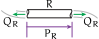
\includegraphics[width=.8\linewidth]{figures/fluid-resistor-R1.pdf}
        &
        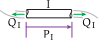
\includegraphics[width=.8\linewidth]{figures/fluid-inertance-I.pdf}
        &
        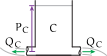
\includegraphics[width=.8\linewidth]{figures/fluid-capacitance-C.pdf}
        \\
        \includegraphics[width=.8\linewidth]{figures/fluid-resistor-R2.pdf} & & 
    \end{tabularx}
    \note[itemize]{
        \item Analogous to the electronic system, for a fluid system, the power flow variables are volumetric flowrate $Q$ and pressure $P$. 
        \item The flowrate is the through-variable and the pressure is the across-variable.
        \item Shown are three common fluid elements: a fluid resistor $R$, an inertance $I$, and a fluid capacitance $C$.
        \item The through- and across-variables of each are shown with subscripts associated with the element.
    }
\end{frame}

\begin{frame}{Thermal power flow variables}
    \begin{equation}
        \underbrace{\mathcal{P}(t)}_{\text{power}} = \underbrace{q(t)}_{\text{through}}.
    \end{equation}
    Also, 
    \begin{equation}
        \underbrace{P(t)}_{\text{across}}.
    \end{equation}
    \hfill\hfill
    \begin{circuitikz}[]
        \draw
          (0,0) to[R=$R$,i=$q_R$,v=$T_R$] (2,0);
    \end{circuitikz}
    \hfill
    \begin{tikzpicture}
        \node[rectangle,draw,thick,rounded corners=.5pt,minimum width=1cm,minimum height=1cm] (m) at (0,0) {$C$};
        \node[groundmech,minimum height=1cm] (g) at (-1.5,0) {};
        \draw (g.south east) -- (g.north east);
        \draw[->,mygreen] (g.north east) -- ++(0,.75)
        -- ++(.3,0)
        node[above] {$T_1$};
        \draw[->,mygreen] (m.north east) -- ++(0,.75)
        -- ++(.3,0)
        node[above] {$T_2$};
        \draw[->,violet] (m.east) -- ++(.5,0)
        node[right] {$q_C$};
        % \draw[fill=white] (0,0) circle (2pt);
        % \draw[fill=white] (2,0) circle (2pt);
    \end{tikzpicture}
    \hfill\hfill
    \note[itemize]{
        \item Surprisingly, thermal systems are a bit different.
        \item Due to the conventional choice of temperature $T$ and heat flowrate $q$ as variables, the power is just the heat flowrate $q$!
        \item However, we do define the across-variable temperature.
        \item The heat flowrate is the through-variable.
        \item Shown are the two common thermal elements: a thermal resistor $R$ and a thermal capacitance $C$.
        \item The through- and across-variables of each are shown with subscripts associated with the element.
    }
\end{frame}

\begin{frame}
\begingroup
\renewcommand*{\arraystretch}{1.85}
\begin{adjustbox}{center}
\tiny
\begin{tabular}{@{}llcccccc@{}}
\toprule
 & & \textbf{generalized} & \begingroup\renewcommand*{\arraystretch}{1}\begin{tabular}[c]{@{}c@{}}\textbf{mechanical}\\ \textbf{translation}\end{tabular}\endgroup & \begingroup\renewcommand*{\arraystretch}{1}\begin{tabular}[c]{@{}c@{}}\textbf{mechanical}\\ \textbf{rotation}\end{tabular}\endgroup & \textbf{electrical} & \textbf{fluid} & \textbf{thermal} \\ 
\cmidrule[\lightrulewidth](lr{1ex}){3-8}%\cmidrule[\lightrulewidth]{3-7}
\multirow{2}{*}{\textbf{variables}} & \emph{across} & $\mathcal{V}$ & velocity $v$ & angular vel.\ $\Omega$ & voltage $v$ & pressure $P$ & temp.\ $T$ \\
% \cmidrule[.5\lightrulewidth](lr{1ex}){2-7}
 & \emph{through} & $\mathcal{F}$ & force $f$ & torque $T$ & current $i$ & vol.\ fr.\ $Q$ & heat fr.\ $q$ \\
\cmidrule[\lightrulewidth](lr{1ex}){3-8}
\multirow{4}{*}{\textbf{A-type}} & \emph{capacitor} & capacitor & mass & mom.\ inertia & capacitor & capacitor & capacitor \\
% \cmidrule[.5\lightrulewidth](lr{1ex}){2-7}
& \emph{capacitance} & $C$ & $m$ & $J$ & $C$ & $C$ & $C$ \\
& \emph{elem.\ eq.} & $\dfrac{d\mathcal{V}_C}{d t} = \dfrac{1}{C} \mathcal{F}_C$ & $\dfrac{d v_m}{d t} = \dfrac{1}{m} f_m$ & $\dfrac{d \Omega_J}{d t} = \dfrac{1}{J} T_J$ & $\dfrac{d v_C}{d t} = \dfrac{1}{C} i_C$ & $\dfrac{d P_C}{d t} = \dfrac{1}{C} Q_C$ & $\dfrac{d T_C}{d t} = \dfrac{1}{C} q_C$ \\
& \emph{impedance} & $\dfrac{1}{C s}$ & $\dfrac{1}{m s}$ & $\dfrac{1}{J s}$ & $\dfrac{1}{C s}$ & $\dfrac{1}{C s}$ & $\dfrac{1}{C s}$ \\
\cmidrule[\lightrulewidth](lr{1ex}){3-8}
\multirow{4}{*}{\textbf{T-type}} & \emph{inductor} & inductor & spring & rot.\ spring& inductor & inertance &  \\
% \cmidrule[.5\lightrulewidth](lr{1ex}){2-6}
& \emph{inductance} & $L$ & $1/k$ & $1/k$ & $L$ & $I$ &  \\
& \emph{elem.\ eq.} & $\dfrac{d\mathcal{F}_L}{d t} = \dfrac{1}{L} \mathcal{V}_L$ & $\dfrac{d f_k}{d t} = k v_k$ & $\dfrac{d T_k}{d t} = k \Omega_k$ & $\dfrac{d i_L}{d t} = \dfrac{1}{L} v_L$ & $\dfrac{d Q_I}{d t} = \dfrac{1}{I} P_I$ & \\
& \emph{impedance} & $L s$ & $s/k$ & $s/k$ & $L s$ & $I s$ &  \\
\cmidrule[\lightrulewidth](lr{1ex}){3-8}
\multirow{4}{*}{\textbf{D-type}} & \emph{resistor} & resistor & damper & rot.\ damper & resistor & resistor & resistor\\
% \cmidrule[.5\lightrulewidth](lr{1ex}){2-7}
& \emph{resistance} & $R$ & $1/B$ & $1/B$ & $R$ & $R$ & $R$ \\ 
& \emph{elem.\ eq.} & $\mathcal{V}_R = \mathcal{F}_R R$ & $v_B = f_B/B$ & $\Omega_B = T_B/B$ & $v_R = i_R R$ & $P_R = Q_R R$ & $T_R = q_R R$ \\
& \emph{impedance} & $R$ & $1/B$ & $1/B$ & $R$ & $R$ & $R$ \\ 
\bottomrule
\end{tabular}
\end{adjustbox}
\endgroup
\end{frame}

%----------------------------------------------------------------------------------------

\end{document}